% ====================================================================
% SINGLE-FILE BUILD - everything inlined. Set this as Main document.
% Put the 12 PNGs in a folder named  figures/  (pdfLaTeX).
% ====================================================================

% ============================================================================
% preamble  —  theme, colours, packages, macros
% Theme switching (e.g. to metropolis) is a one-line change on \usetheme below.
% ============================================================================
\documentclass[aspectratio=169,11pt]{beamer}

\usetheme{Madrid}
\usecolortheme{default}

% ---- Daylight-projector contrast: darken the Madrid blue (piraeusblue) -------
\definecolor{piraeusblue}{RGB}{20,40,90}
\definecolor{piraeuslight}{RGB}{74,111,165}
\definecolor{piraeusaccent}{RGB}{184,134,11}   % dark goldenrod, "winner" highlight
\definecolor{softgrey}{RGB}{154,163,173}
\definecolor{panelbg}{RGB}{238,242,248}
\definecolor{goodgreen}{RGB}{46,125,50}

\setbeamercolor{structure}{fg=piraeusblue}
\setbeamercolor{frametitle}{bg=piraeusblue,fg=white}
\setbeamercolor{title}{fg=piraeusblue}
\setbeamercolor{palette primary}{bg=piraeusblue,fg=white}
\setbeamercolor{palette secondary}{bg=piraeuslight,fg=white}
\setbeamercolor{palette tertiary}{bg=piraeusblue,fg=white}
\setbeamercolor{block title}{bg=piraeusblue,fg=white}
\setbeamercolor{block body}{bg=panelbg,fg=black}
\setbeamercolor{itemize item}{fg=piraeusblue}
\setbeamercolor{itemize subitem}{fg=piraeuslight}

% Cleaner frame titles, no shadow; remove navigation clutter.
\setbeamertemplate{frametitle}[default][colsep=-4bp,rounded=false]
\setbeamertemplate{navigation symbols}{}
\setbeamertemplate{itemize items}[circle]
\setbeamertemplate{blocks}[rounded][shadow=false]
\setbeamerfont{frametitle}{series=\bfseries}

% ---- Packages ---------------------------------------------------------------
\usepackage[english]{babel}
\usepackage{graphicx}
\usepackage{booktabs}
\usepackage{tikz}
\usepackage{caption}
\captionsetup{font=footnotesize,labelfont=bf}

\usetikzlibrary{arrows.meta,positioning,calc,fit,backgrounds}

% ---- Number / naming macros -------------------------------------------------
\newcommand{\macroF}[1]{\textbf{#1}}                         % bold headline F1
\newcommand{\best}[1]{\textcolor{piraeusaccent}{\textbf{#1}}} % winner highlight
\newcommand{\arch}[1]{\textsc{#1}}
\newcommand{\source}[1]{{\footnotesize\itshape\textcolor{softgrey}{#1}}}
\newcommand{\num}[1]{#1}

% Tight itemize spacing
\setlength{\leftmargini}{1.4em}
\setbeamertemplate{itemize/enumerate body begin}{\small}

% ---- Footline fix -----------------------------------------------------------
% FORMATTING FIX (footer overflow): the default Madrid/infolines footline packs
% short-author + (institute) into a fixed .333\paperwidth box. With this author
% list + institute the left box overflows ~37pt, clipping the author at the page
% edge and overlapping the institute into the title box. Rebalanced box widths
% (.44 / .32 / .24) keep all three surnames + title + date/frame legible on one
% line. The institute parenthetical is dropped from the FOOTER only; it still
% appears in full on the title slide via \insertinstitute. No text changed.
\setbeamertemplate{footline}{%
  \leavevmode\hbox{%
  \begin{beamercolorbox}[wd=.44\paperwidth,ht=2.25ex,dp=1ex,center]{author in head/foot}%
    \usebeamerfont{author in head/foot}\insertshortauthor%
  \end{beamercolorbox}%
  \begin{beamercolorbox}[wd=.32\paperwidth,ht=2.25ex,dp=1ex,center]{title in head/foot}%
    \usebeamerfont{title in head/foot}\insertshorttitle%
  \end{beamercolorbox}%
  \begin{beamercolorbox}[wd=.24\paperwidth,ht=2.25ex,dp=1ex,leftskip=1.5ex,rightskip=1.5ex,sep=0pt]{date in head/foot}%
    \hfill\usebeamerfont{date in head/foot}\insertshortdate{}\hfill%
    \usebeamercolor[fg]{page number in head/foot}\usebeamerfont{page number in head/foot}%
    \usebeamertemplate{page number in head/foot}%
  \end{beamercolorbox}}\vskip0pt}

% ---- Figure path ------------------------------------------------------------
\graphicspath{{figures/}{./}}


% ===== metadata =====
% ============================================================================
% metadata  —  title, author, institute, date
% ============================================================================
\title[CIFAR-100 Architectures]{Deep Learning Image Classification on CIFAR-100}
\subtitle{Sequence baselines, CNN controls, transfer learning, and HF ViT}

\author[Grammatikopoulos, Dimopoulos, Kokkas]{%
  Faidon Grammatikopoulos \and Konstantinos Dimopoulos \and Theodoros Kokkas}

\institute[NCSR Demokritos \& UniPi]{%
  MSc in Artificial Intelligence\\
  NCSR ``Demokritos'' \& University of Piraeus\\
  Deep Learning Course
}

% NOTE: replace with the actual presentation date before producing the final PDF.
\date{June 2026}


\begin{document}


% ----- 01 Title -----
\begin{frame}[plain]
  \centering
  \vspace{1.4em}
  \begin{beamercolorbox}[wd=\paperwidth,sep=16pt,center]{palette primary}
    {\usebeamerfont{title}\bfseries\inserttitle\par}
    \vspace{0.45em}
    {\small\insertsubtitle\par}
  \end{beamercolorbox}
  \vfill
  {\large\insertauthor\par}
  \vspace{1.0em}
  {\footnotesize\insertinstitute\par}
  \vspace{1.4em}
  {\insertdate\par}
  \vfill
\end{frame}


% ----- 02 CIFAR-100 task framing -----
\begin{frame}{CIFAR-100: one dataset, two label hierarchies}
  \begin{columns}[T,onlytextwidth]
    \column{0.56\textwidth}
      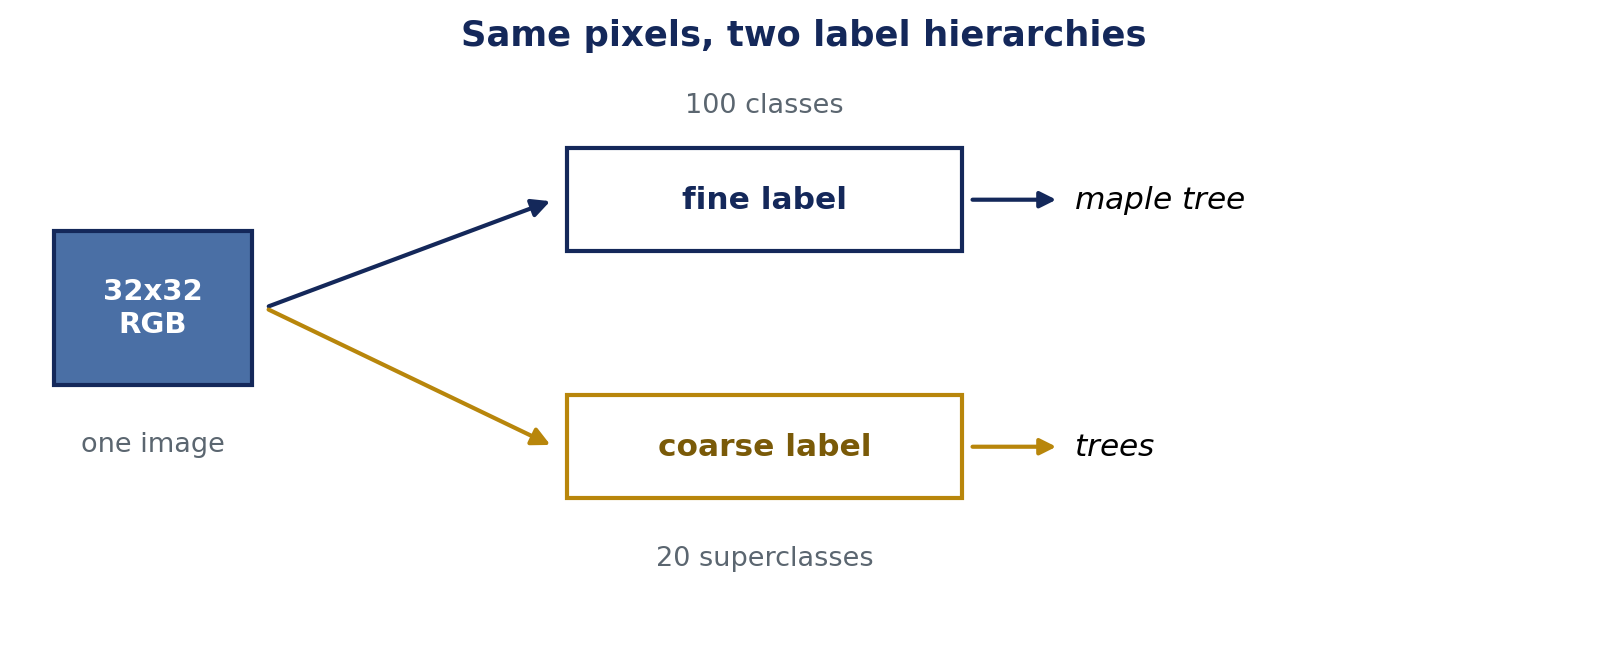
\includegraphics[width=\linewidth]{label_hierarchy.png}
    \column{0.42\textwidth}
      \begin{itemize}
        \item \num{60000} natural images, only \textbf{32$\times$32} RGB --- very little
              signal per sample.
        \item Every image carries a \textbf{fine} label (100 classes) nested inside a
              \textbf{coarse} superclass (20 classes).
        \item We study three task styles on the \emph{same} pixels:
              \emph{binary} one-vs-rest, \emph{coarse} 20-class, \emph{fine} 100-class.
      \end{itemize}
  \end{columns}
  \vfill
  \source{Standard 50k train / 10k test split, \texttt{uoft-cs/cifar100}.}
\end{frame}


% ----- 03 Research question -----
\begin{frame}{Research question}
  \vfill
  \begin{block}{}
    \centering\large
    How do different \textbf{architecture families} compare on CIFAR-100
    under \textbf{limited data} and a \textbf{32$\times$32} input, and how far does
    \textbf{transfer learning} move beyond from-scratch baselines?
  \end{block}
  \vfill
  \begin{itemize}
    \item A \emph{comparison} study, not a single-model study: sequence models, compact and
          stronger CNN controls, pretrained CNN families, and a transformer notebook.
    \item Held constant across families: the data splits, the evaluation protocol, and
          \textbf{Macro F1} as the primary metric.
    \item What varies: backbone capacity, and how much of it we unfreeze.
  \end{itemize}
  \vfill
\end{frame}


% ----- 04 Experimental setup -----
\begin{frame}{Experimental setup}
  \centering
  \renewcommand{\arraystretch}{1.25}
  \begin{tabular}{@{}ll@{}}
    \toprule
    \textbf{Aspect} & \textbf{Choice} \\
    \midrule
    Data            & CIFAR-100, 50k train / 10k test, 32$\times$32 RGB \\
    Validation      & 10\% split off the training set \\
    Tasks           & binary (1-vs-rest) $\cdot$ coarse (20) $\cdot$ fine (100) \\
    Primary metric  & \textbf{Macro F1} \;(+ Top-5 accuracy for multiclass) \\
    Transfer regimes& frozen head $\rightarrow$ partial unfreeze $\rightarrow$ full fine-tune \\
    Optimiser       & Adam; light augmentation where configured \\
    Input handling  & Scratch at 32 px; EfficientNet at 96--160 px; other transfer / ViT at 224 px \\
    Compute         & Google Colab T4 GPU; fixed seed 42 \\
    \bottomrule
  \end{tabular}

  \vfill
  \begin{itemize}
    \item Macro F1 weights every class equally, so it stays honest on the
          \emph{balanced} 20- and 100-class tasks \emph{and} on the severely
          imbalanced 1-vs-rest tasks, where high accuracy can hide poor positive-class recall.
  \end{itemize}
\end{frame}


% ----- 05 Architecture families surveyed -----
\begin{frame}{Architecture families surveyed}
  \centering
  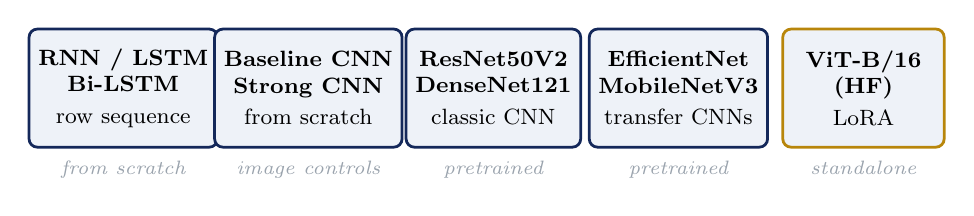
\begin{tikzpicture}[
      box/.style={draw=piraeusblue,line width=1pt,rounded corners=3pt,
                  fill=panelbg,minimum width=2.05cm,minimum height=1.5cm,
                  align=center,font=\footnotesize},
      lbl/.style={font=\scriptsize\itshape,text=softgrey},
      x=2.35cm]
    \node[box] (a) at (0,0) {\textbf{RNN / LSTM}\\\textbf{Bi-LSTM}\\[2pt]row sequence};
    \node[box] (b) at (1,0) {\textbf{Baseline CNN}\\\textbf{Strong CNN}\\[2pt]from scratch};
    \node[box] (c) at (2,0) {\textbf{ResNet50V2}\\\textbf{DenseNet121}\\[2pt]classic CNN};
    \node[box] (d) at (3,0) {\textbf{EfficientNet}\\\textbf{MobileNetV3}\\[2pt]transfer CNNs};
    \node[box,draw=piraeusaccent] (e) at (4,0)
        {\textbf{ViT-B/16}\\\textbf{(HF)}\\[2pt]LoRA};
    \node[lbl,below=1pt of a] {from scratch};
    \node[lbl,below=1pt of b] {image controls};
    \node[lbl,below=1pt of c] {pretrained};
    \node[lbl,below=1pt of d] {pretrained};
    \node[lbl,below=1pt of e] {standalone};
  \end{tikzpicture}

  \vfill
  \begin{columns}[T,onlytextwidth]
    \column{0.62\textwidth}
      \begin{itemize}
        \item The local code compares \textbf{row-sequence models}, from-scratch CNN
              controls, and several pretrained image backbones.
        \item Pretrained backbones are evaluated under frozen, partially unfrozen, or
              fine-tuned regimes when the corresponding runs exist.
      \end{itemize}
    \column{0.36\textwidth}
      \begin{block}{Narrative arc}
        \footnotesize From-scratch controls $\rightarrow$ transfer lift $\rightarrow$
        transformer transfer.
      \end{block}
  \end{columns}
\end{frame}


% ----- 06 Why accuracy misleads under imbalance -----
\begin{frame}{Warm-up: why accuracy misleads under imbalance}
  \begin{columns}[T,onlytextwidth]
    \column{0.62\textwidth}
      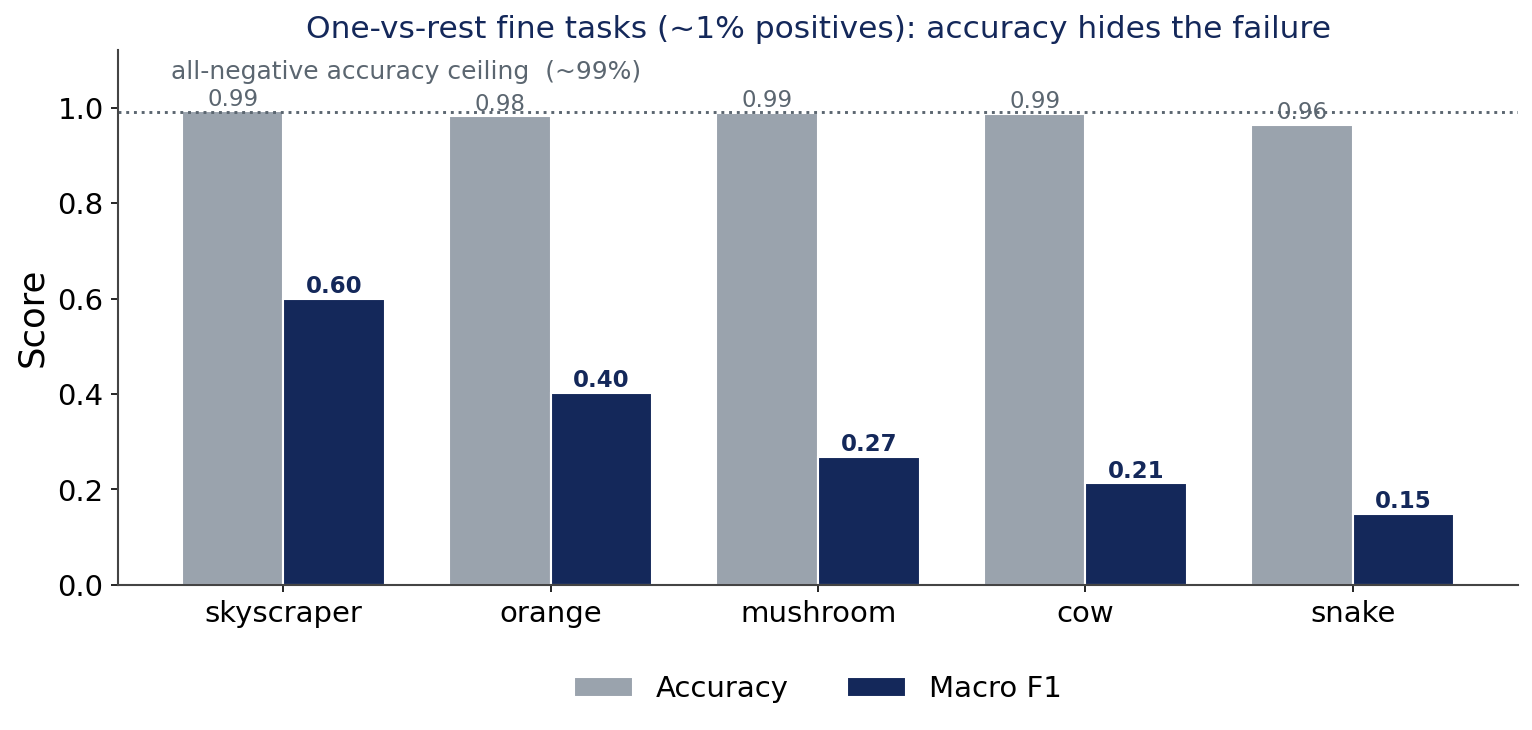
\includegraphics[width=\linewidth]{binary_accuracy_vs_f1_gap.png}
    \column{0.36\textwidth}
      \begin{itemize}
        \item A fine class is $\sim$\textbf{1\%} of the data, so predicting
              ``always negative'' already scores $\sim$\textbf{99\%} accuracy.
        \item The baseline CNN sits near that ceiling on every task, yet Macro F1
              ranges from \textbf{0.60} (skyscraper) down to \textbf{0.15} (snake).
        \item Accuracy hides the failure; \textbf{Macro F1} exposes it. This is why
              it is our primary metric everywhere that follows.
      \end{itemize}
  \end{columns}
  \vfill
  \source{Best baseline-CNN run per one-vs-rest fine task (results/*/metrics.json).}
\end{frame}


% ----- 07 From-scratch controls on 20 coarse classes -----
\begin{frame}{From-scratch controls on 20 coarse classes}
  \centering
  \renewcommand{\arraystretch}{1.18}
  \begin{tabular}{@{}lcccc@{}}
    \toprule
    \textbf{Run} & \textbf{Input view} & \textbf{Accuracy} & \textbf{Macro F1} & \textbf{Top-5} \\
    \midrule
    Baseline CNN & image $(32,32,3)$ & 0.281 & 0.263 & 0.662 \\
    Strong CNN, regularized + aug. & image $(32,32,3)$ & 0.283 & 0.274 & 0.656 \\
    LSTM sequence & rows $(32,96)$ & 0.329 & 0.311 & 0.720 \\
    Bi-LSTM sequence & rows $(32,96)$ & \best{0.356} & \best{0.345} & \best{0.741} \\
    \bottomrule
  \end{tabular}

  \vfill
  \begin{itemize}
    \item The sequence models are useful \textbf{from-scratch controls}: they read each
          image as 32 row-timesteps with 96 features per row.
    \item The stronger CNN improved over the compact baseline, but did not close the gap
          to LSTM/Bi-LSTM in this recorded coarse run.
    \item This is a project-specific baseline finding, not a claim that recurrent models
          are generally stronger image classifiers than CNNs.
  \end{itemize}
  \vfill
  \source{Local results: baseline CNN, strong CNN, LSTM, and Bi-LSTM coarse multiclass metrics.}
\end{frame}


% ----- 08 Coarse: transfer learning lifts the floor -----
\begin{frame}{Coarse: transfer learning lifts the floor}
  \centering
  % fmt: height cap keeps image + bullet columns clear of the footer
  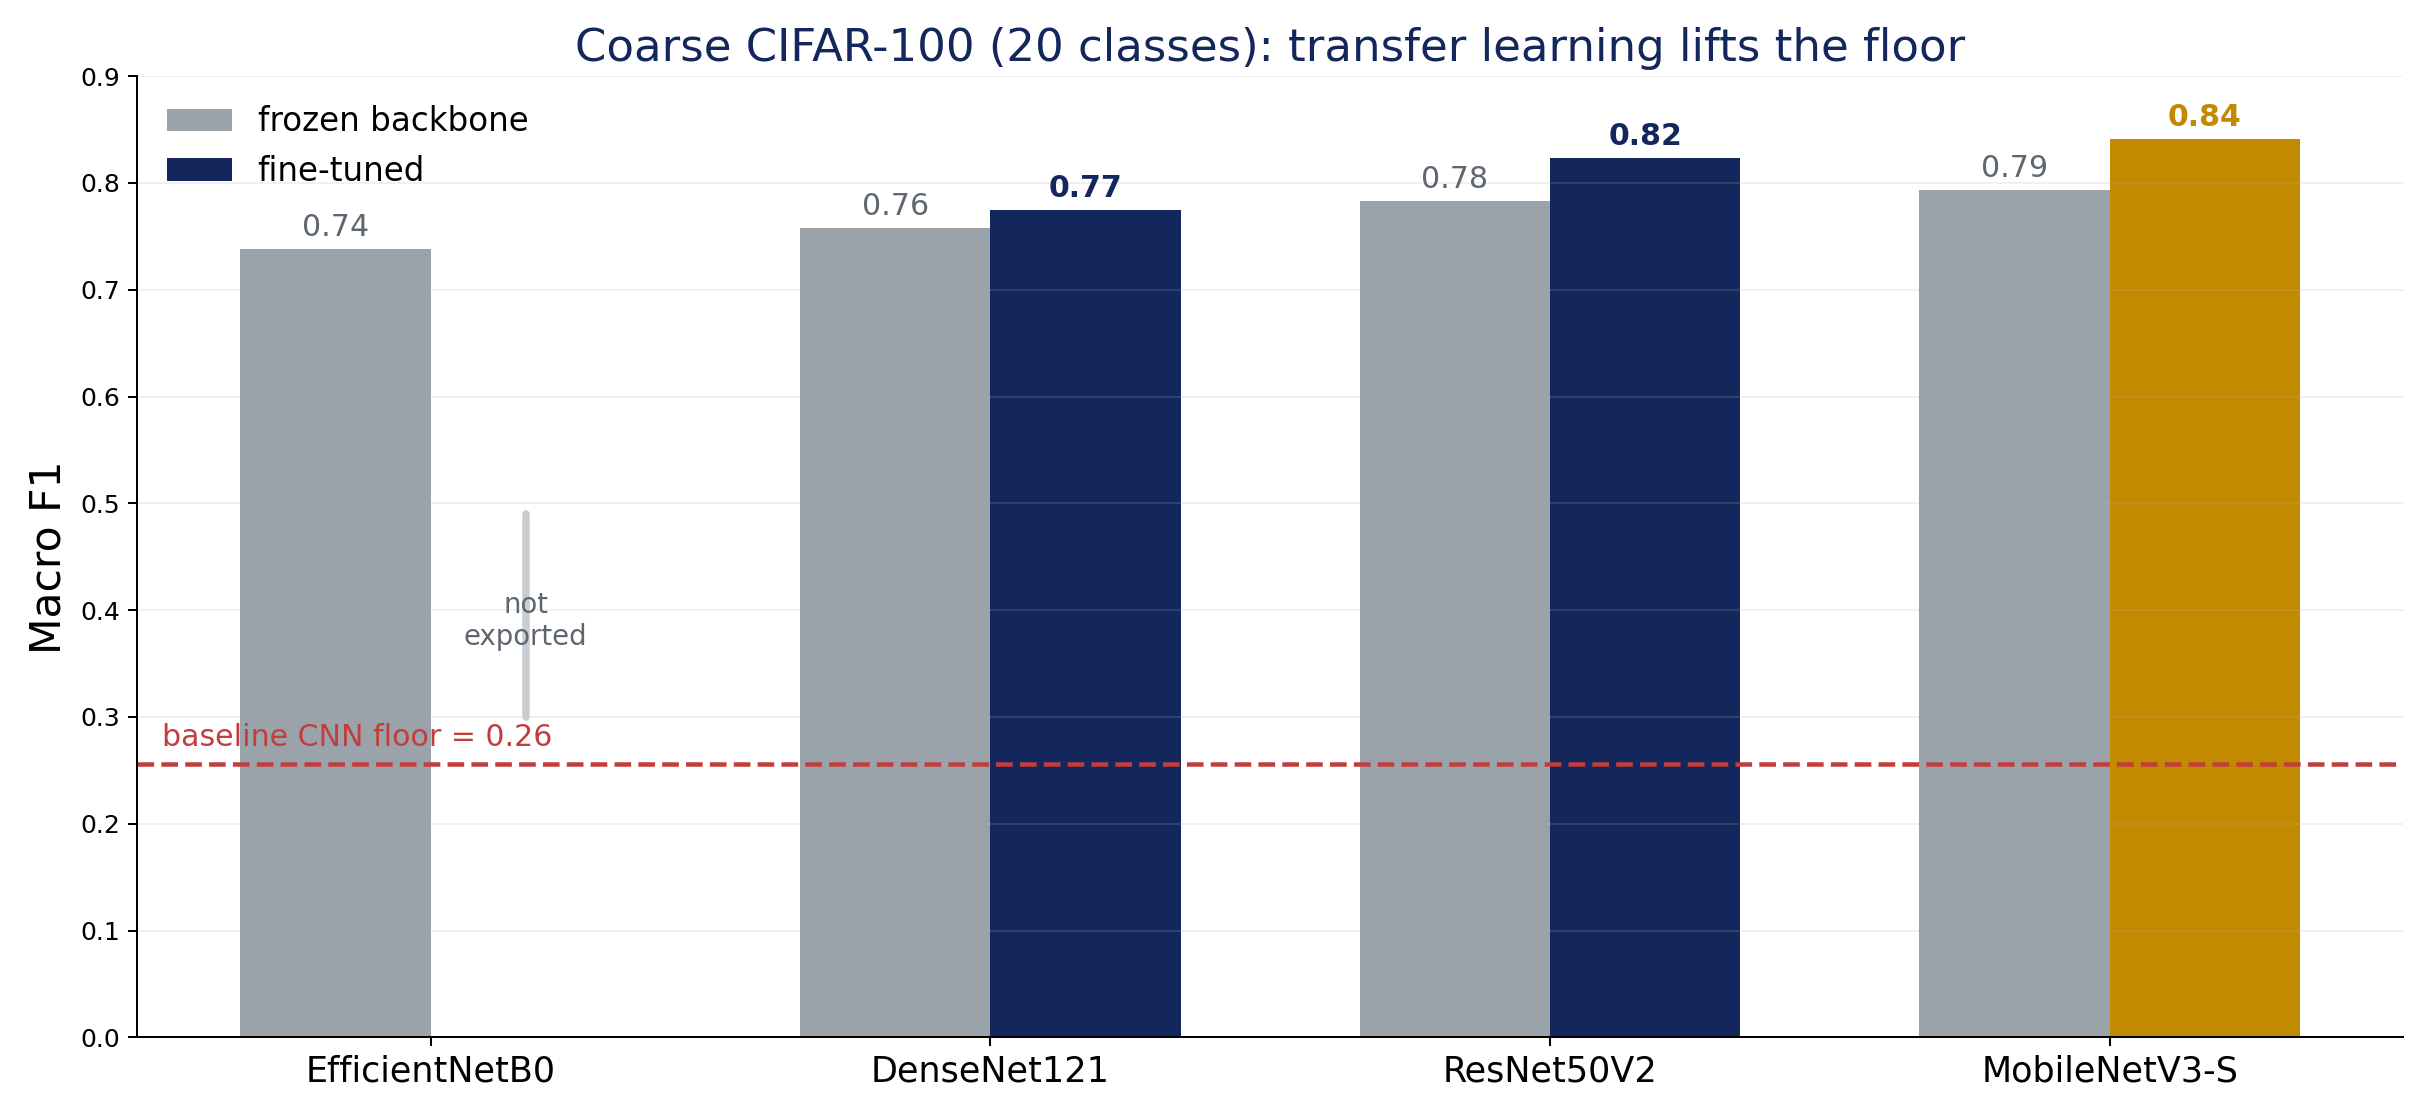
\includegraphics[width=0.84\linewidth,height=0.52\textheight,keepaspectratio]{coarse_transfer_macro_f1.png}\\[0.4em]
  \begin{columns}[T,onlytextwidth]
    \column{0.49\textwidth}
      \begin{itemize}
        \item Every pretrained backbone clears the \textbf{0.26} baseline by a wide margin,
              landing in the \textbf{0.74--0.84} Macro F1 band.
      \end{itemize}
    \column{0.49\textwidth}
      \begin{itemize}
        \item Unfreezing helps consistently: fine-tuning beats the frozen head for
              every family where both regimes were run.
      \end{itemize}
  \end{columns}
  \vfill
  \source{ResNet50V2 / DenseNet121 / EfficientNetB0 / MobileNetV3-Small, coarse multiclass. EfficientNetB0 coarse fine-tune was not exported.}
\end{frame}


% ----- 09 Coarse best: MobileNetV3-Small unfrozen -----
\begin{frame}{Coarse winner: MobileNetV3-Small, fully unfrozen}
  \begin{columns}[T,onlytextwidth]
    \column{0.58\textwidth}
      % fmt: height cap stops the square matrix from running into the footer
      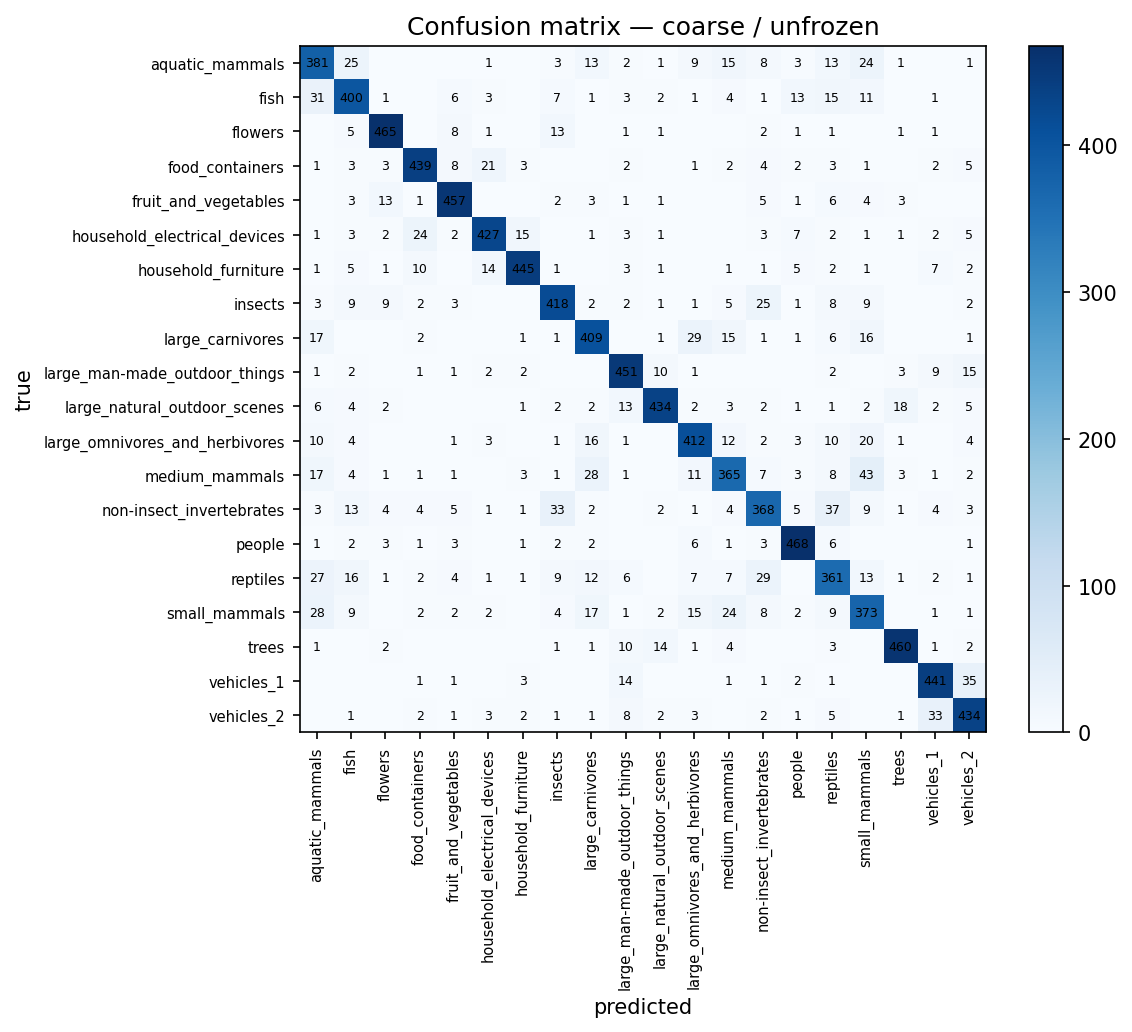
\includegraphics[width=\linewidth,height=0.72\textheight,keepaspectratio]{mobilenetv3_coarse_confusion.png}
    \column{0.40\textwidth}
      \begin{itemize}
        \item \best{Macro F1 = 0.8409}, Top-5 \textbf{0.983} --- the best coarse
              result of the study.
        \item The lightest \emph{pretrained} backbone (2.5\,M params) wins coarse once
              fully unfrozen (+0.047 over its frozen head).
        \item A strong, mostly-diagonal confusion matrix; residual errors fall between
              semantically close superclasses.
      \end{itemize}
  \end{columns}
  \vfill
  \source{nb06 MobileNetV3-Small, coarse, unfrozen (results/mobilenetv3\_coarse/).}
\end{frame}


% ----- 10 Fine task: why 100 classes is harder -----
\begin{frame}{Fine task: why 100 classes is harder}
  \begin{columns}[T,onlytextwidth]
    \column{0.60\textwidth}
      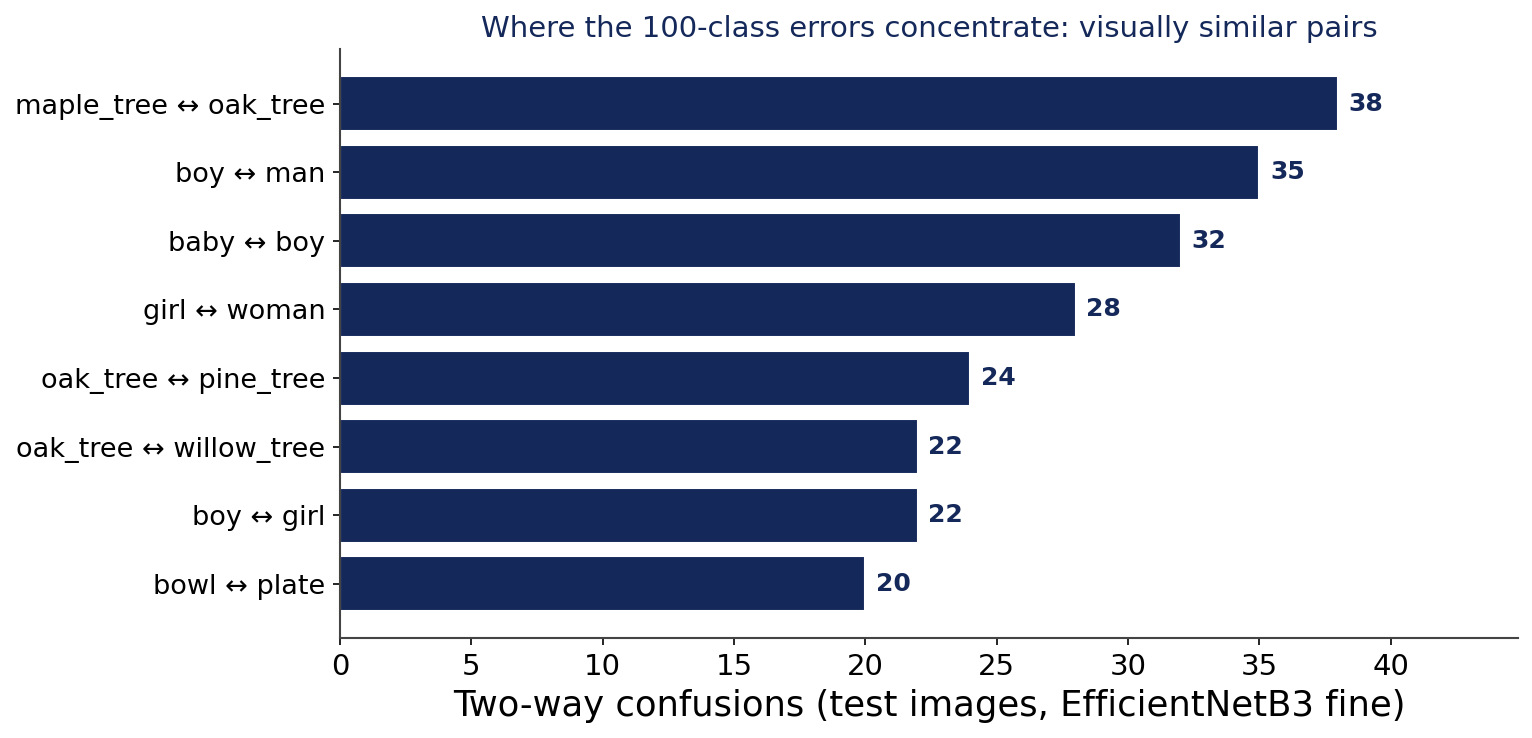
\includegraphics[width=\linewidth]{fine_confusion_pairs.png}
    \column{0.38\textwidth}
      \begin{itemize}
        \item \textbf{5$\times$ more classes} on the same 32$\times$32 input: the decision
              boundary gets far finer.
        \item Errors are not random --- they \textbf{concentrate within superclasses}:
              \emph{maple$\leftrightarrow$oak}, \emph{boy$\leftrightarrow$man},
              \emph{girl$\leftrightarrow$woman}.
        \item So the fine problem is really about separating \emph{visually similar}
              members of the same coarse group.
      \end{itemize}
  \end{columns}
  \vfill
  \source{Two-way confusions from the EfficientNetB3 fine confusion matrix.}
\end{frame}


% ----- 11 EfficientNetB0 fine: frozen -> block6 -> full -----
\begin{frame}{EfficientNetB0 fine: how far unfreezing goes}
  \centering
  % fmt: height cap keeps image + bullet columns clear of the footer
  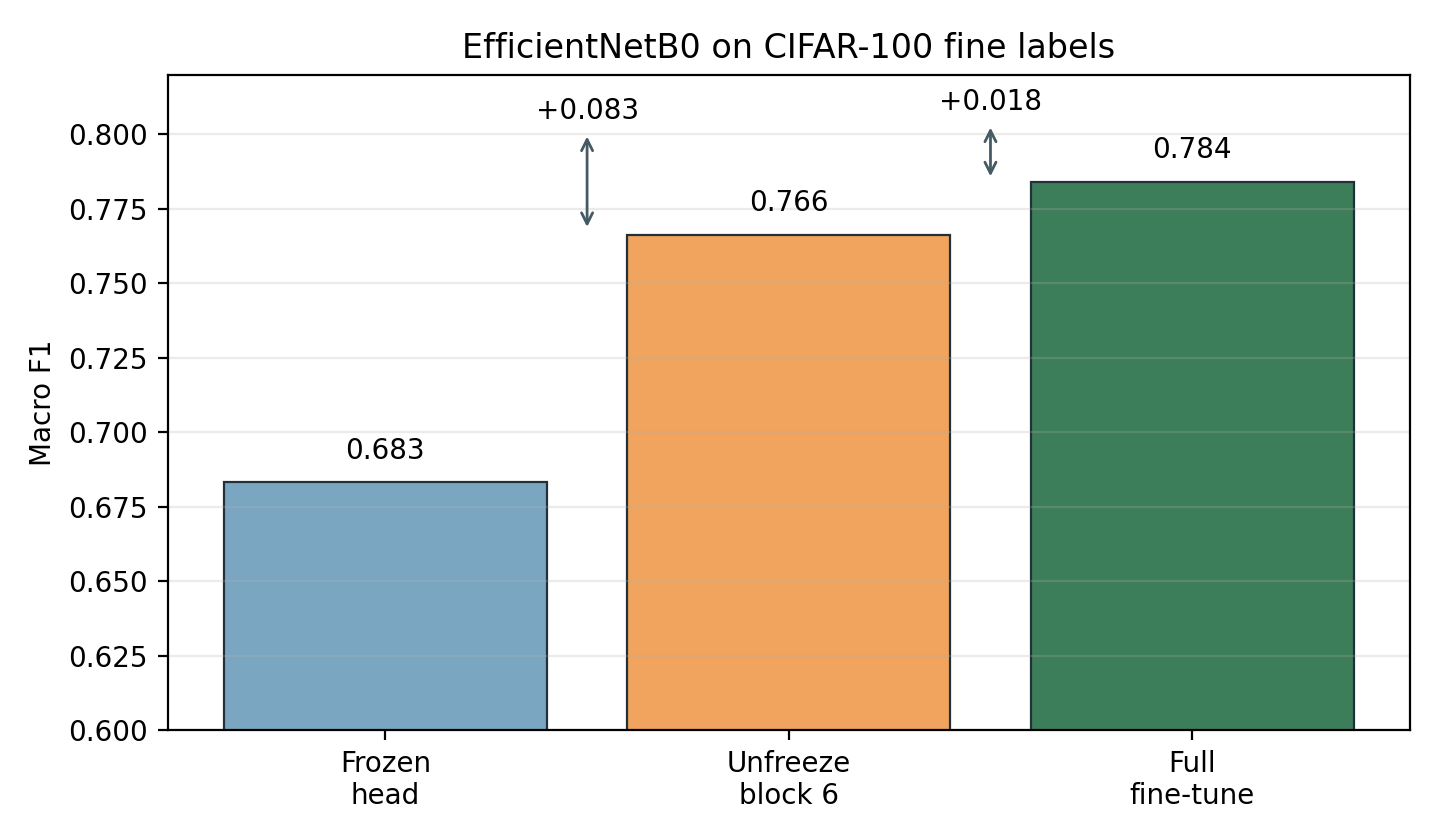
\includegraphics[width=0.72\linewidth,height=0.52\textheight,keepaspectratio]{efficientnetb0_fine_progression.png}\\[0.3em]
  \begin{columns}[T,onlytextwidth]
    \column{0.49\textwidth}
      \begin{itemize}
        \item Frozen head already reaches \textbf{0.683}; unfreezing block 6 adds
              \textbf{+0.083}, full fine-tune a further \textbf{+0.018}.
      \end{itemize}
    \column{0.49\textwidth}
      \begin{itemize}
        \item \textbf{+0.101 Macro F1} end-to-end --- the largest frozen$\to$tuned lift of any
              family, and the template for the B3 run next.
      \end{itemize}
  \end{columns}
  \vfill
  \source{nb05 EfficientNetB0 fine, input 128 (frozen / unfreeze block6 / full ft).}
\end{frame}


% ----- 12 Fine best ConvNet: EfficientNetB3 full fine-tune -----
\begin{frame}{Best fine ConvNet: EfficientNetB3, full fine-tune}
  \begin{columns}[T,onlytextwidth]
    \column{0.60\textwidth}
      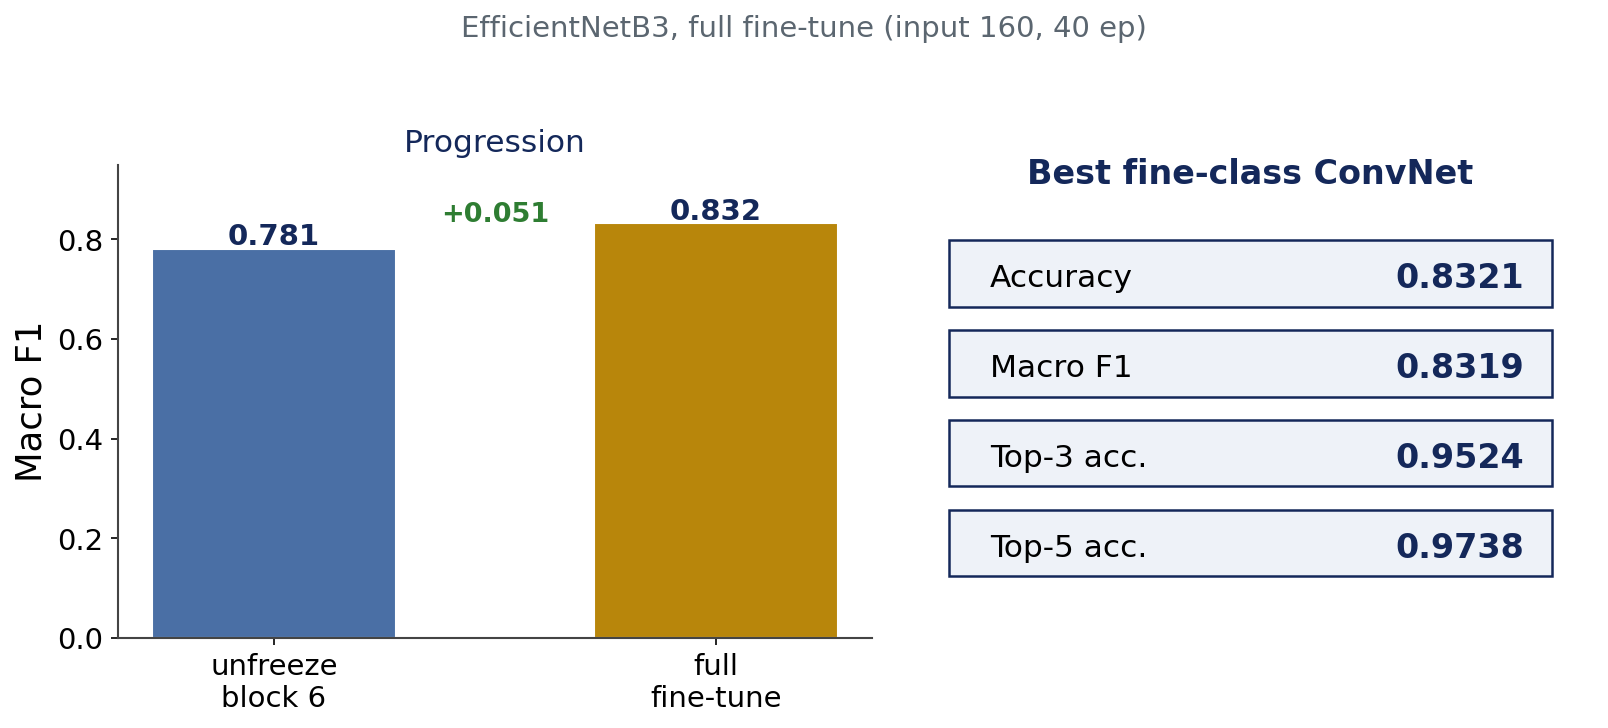
\includegraphics[width=\linewidth]{efficientnetb3_fine_summary.png}
    \column{0.38\textwidth}
      \begin{itemize}
        \item \best{Macro F1 = 0.8319}, Top-5 \textbf{0.974} --- the strongest
              \emph{convolutional} fine result.
        \item A larger pretrained backbone (12.3\,M) plus a larger input (160\,px)
              closes much of the 100-class gap.
        \item Clear winner among the TensorFlow/Keras ConvNet fine multiclass runs.
      \end{itemize}
  \end{columns}
  \vfill
  \source{nb08 EfficientNetB3 fine, full fine-tune, input 160, 40 epochs.}
\end{frame}


% ----- 13 HF ViT-B/16: transformer transfer workflow -----
\begin{frame}{HF ViT-B/16: transformer transfer workflow}
  \begin{columns}[T,onlytextwidth]
    \column{0.58\textwidth}
      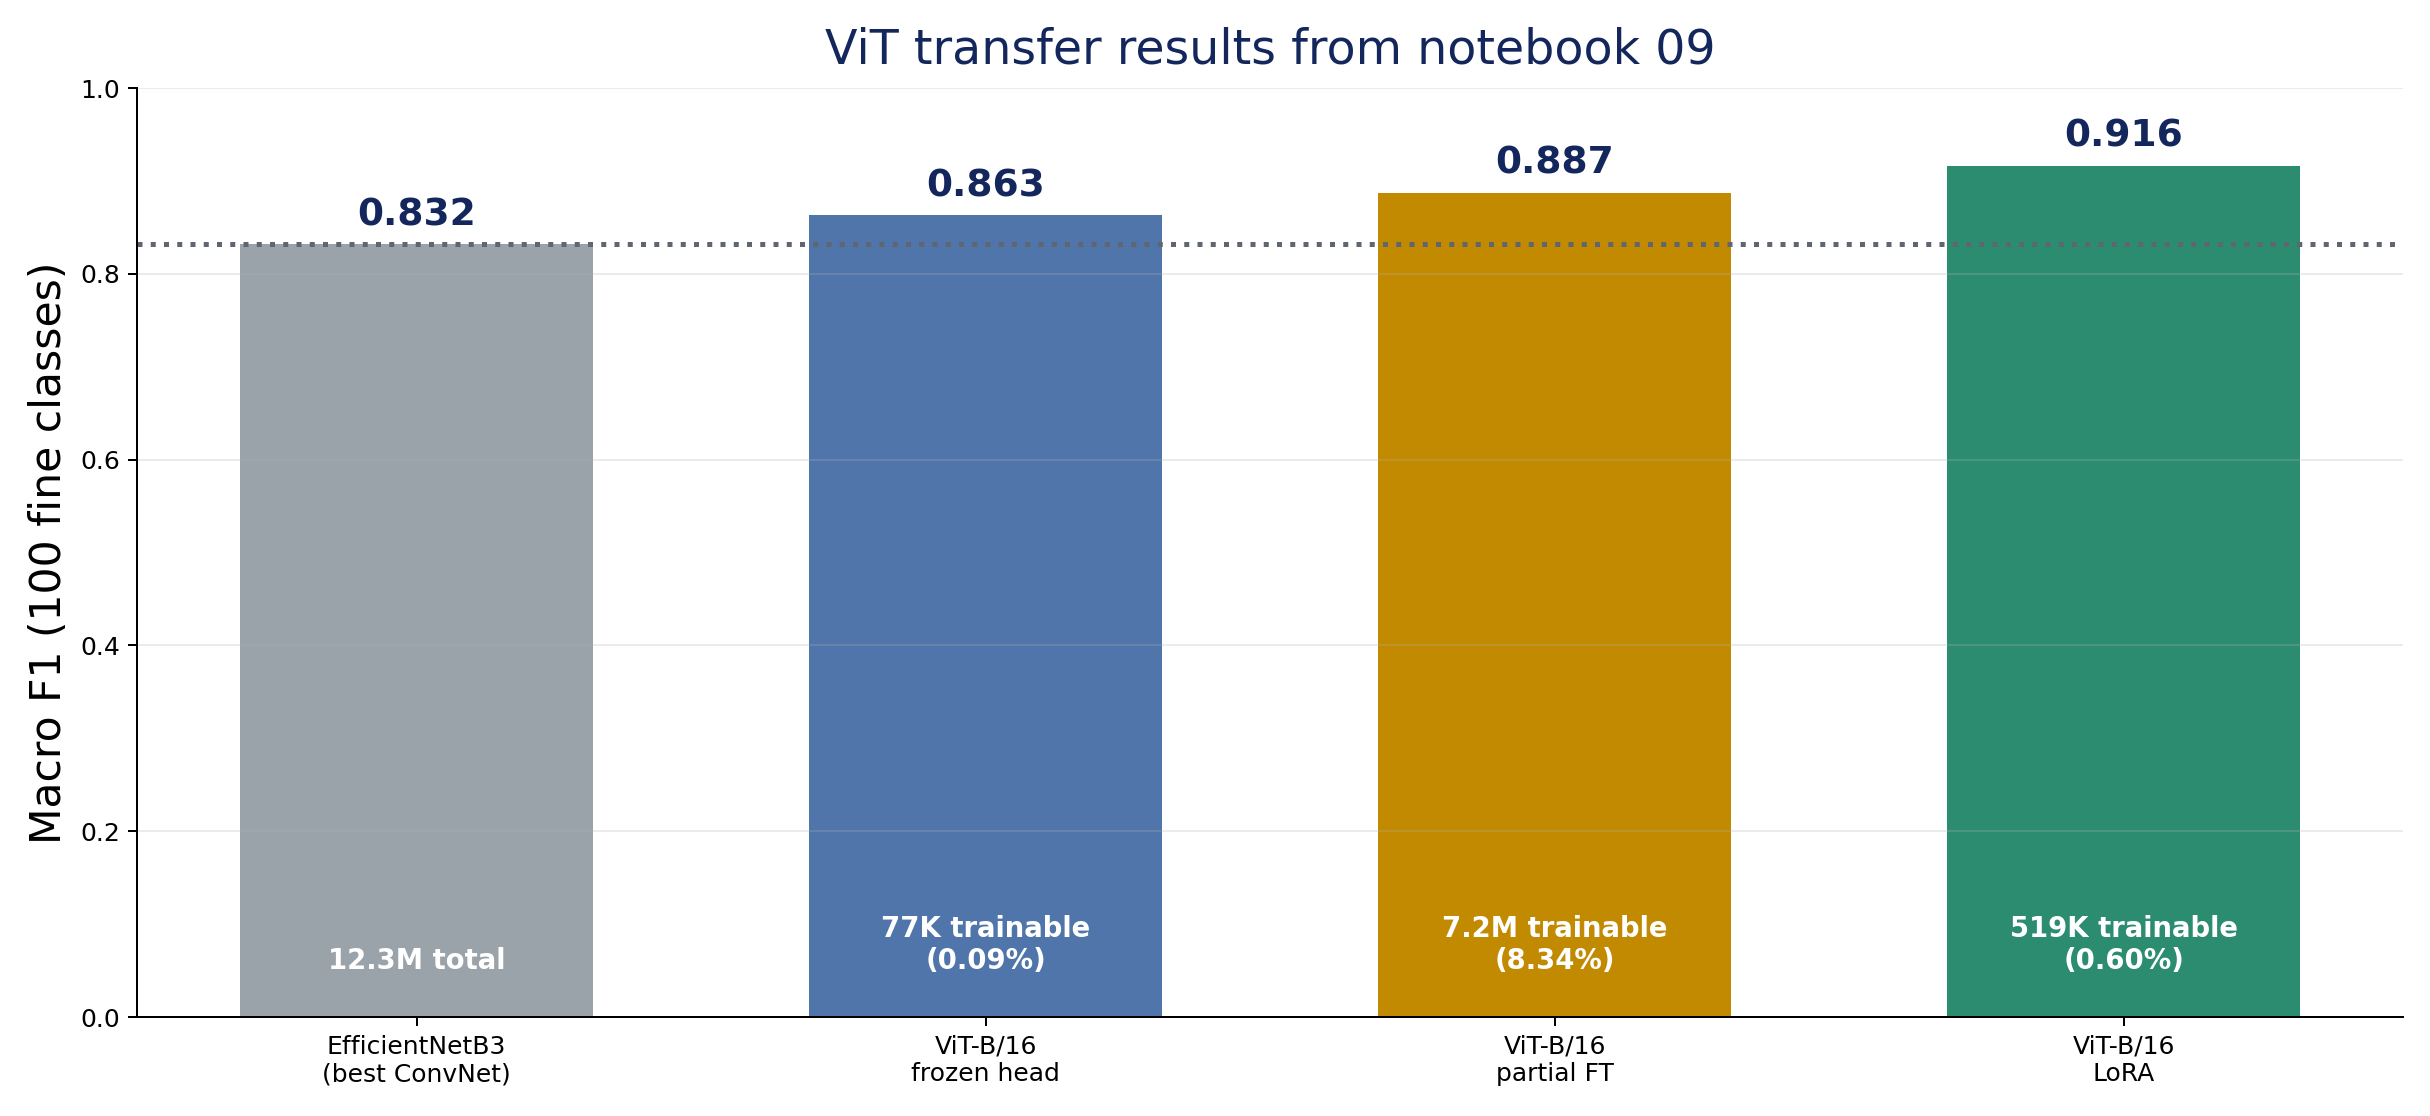
\includegraphics[width=\linewidth]{hf_vit_training_summary.png}
    \column{0.40\textwidth}
      \textbf{Notebook 09 results}
      \begin{itemize}
        \item Frozen head: \macroF{0.8629} Macro F1.
        \item Partial fine-tune: \macroF{0.8873} Macro F1.
        \item LoRA: \best{0.9165} Macro F1, Top-5 \textbf{0.9919}.
        \item Different stack: PyTorch, Transformers, HF processor at 224\,px.
      \end{itemize}
  \end{columns}
  \vfill
  \source{nb09 Hugging Face ViT notebook, CIFAR-100 fine test split.}
\end{frame}


% ----- 14 Transformer caveats -----
\begin{frame}{Transformer caveats: how to compare ViT fairly}
  \begin{columns}[T,onlytextwidth]
    \column{0.48\textwidth}
      \begin{block}{Best fine result}
        \centering
        \Large \textbf{ViT-B/16 + LoRA}\\[0.3em]
        \macroF{Macro F1 = 0.9165}\\
        Top-5 = 0.9919
      \end{block}
    \column{0.48\textwidth}
      \begin{itemize}
        \item ViT changes more than the architecture: the processor resizes CIFAR-100 from
              32$\times$32 to 224$\times$224 and applies transformer-specific normalization.
        \item The strongest ConvNet result remains \textbf{EfficientNetB3} with
              Macro F1 \textbf{0.8319}; ViT moves the ceiling higher.
        \item The comparison is meaningful on the same CIFAR-100 test labels, but the
              framework, input size, and pretraining prior are different.
      \end{itemize}
  \end{columns}
  \vfill
  \source{nb09 ViT results; nb08 EfficientNetB3 result for the ConvNet reference.}
\end{frame}


% ----- 15 Frozen vs fine-tuned: when does unfreezing pay off? -----
\begin{frame}{When does unfreezing or PEFT pay off?}
  \centering
  % fmt: height cap keeps image + bullet columns clear of the footer
  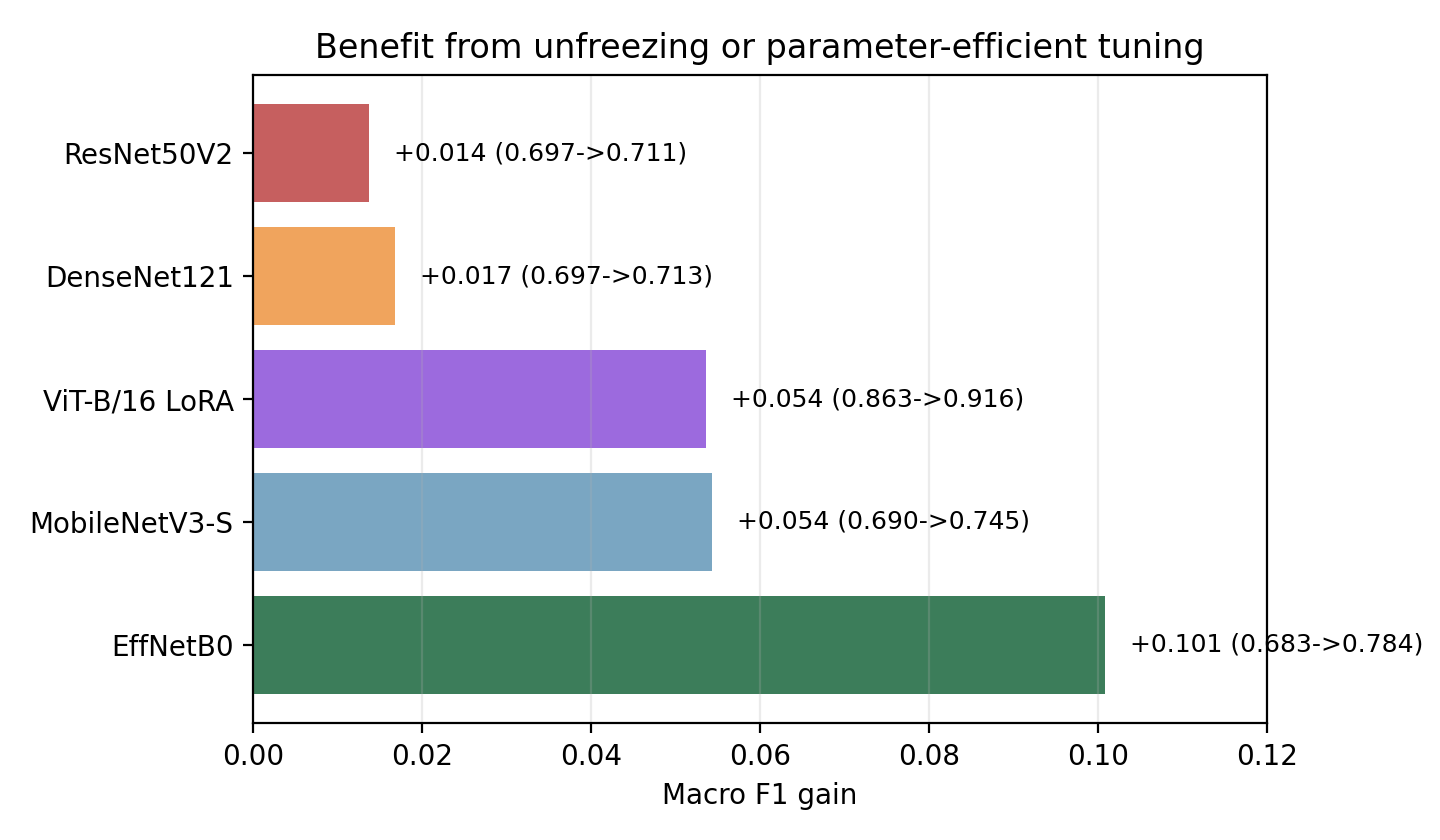
\includegraphics[width=0.72\linewidth,height=0.52\textheight,keepaspectratio]{frozen_to_finetuned_delta.png}\\[0.3em]
  \begin{columns}[T,onlytextwidth]
    \column{0.49\textwidth}
      \begin{itemize}
        \item Unfreezing helps the fine task for the families where frozen and tuned
              results were both exported.
      \end{itemize}
    \column{0.49\textwidth}
      \begin{itemize}
        \item Largest ConvNet gain: \textbf{EfficientNetB0} ($0.683\rightarrow0.784$);
              MobileNetV3-S and ViT-LoRA both add about \textbf{+0.054}.
      \end{itemize}
  \end{columns}
  \vfill
  \source{Per-architecture frozen/head-only $\rightarrow$ best tuned Macro F1 (fine task). ViT uses LoRA, not layer unfreezing.}
\end{frame}


% ----- 16 Compute vs accuracy trade-off -----
\begin{frame}{Compute vs.\ accuracy trade-off}
  \begin{columns}[T,onlytextwidth]
    \column{0.62\textwidth}
      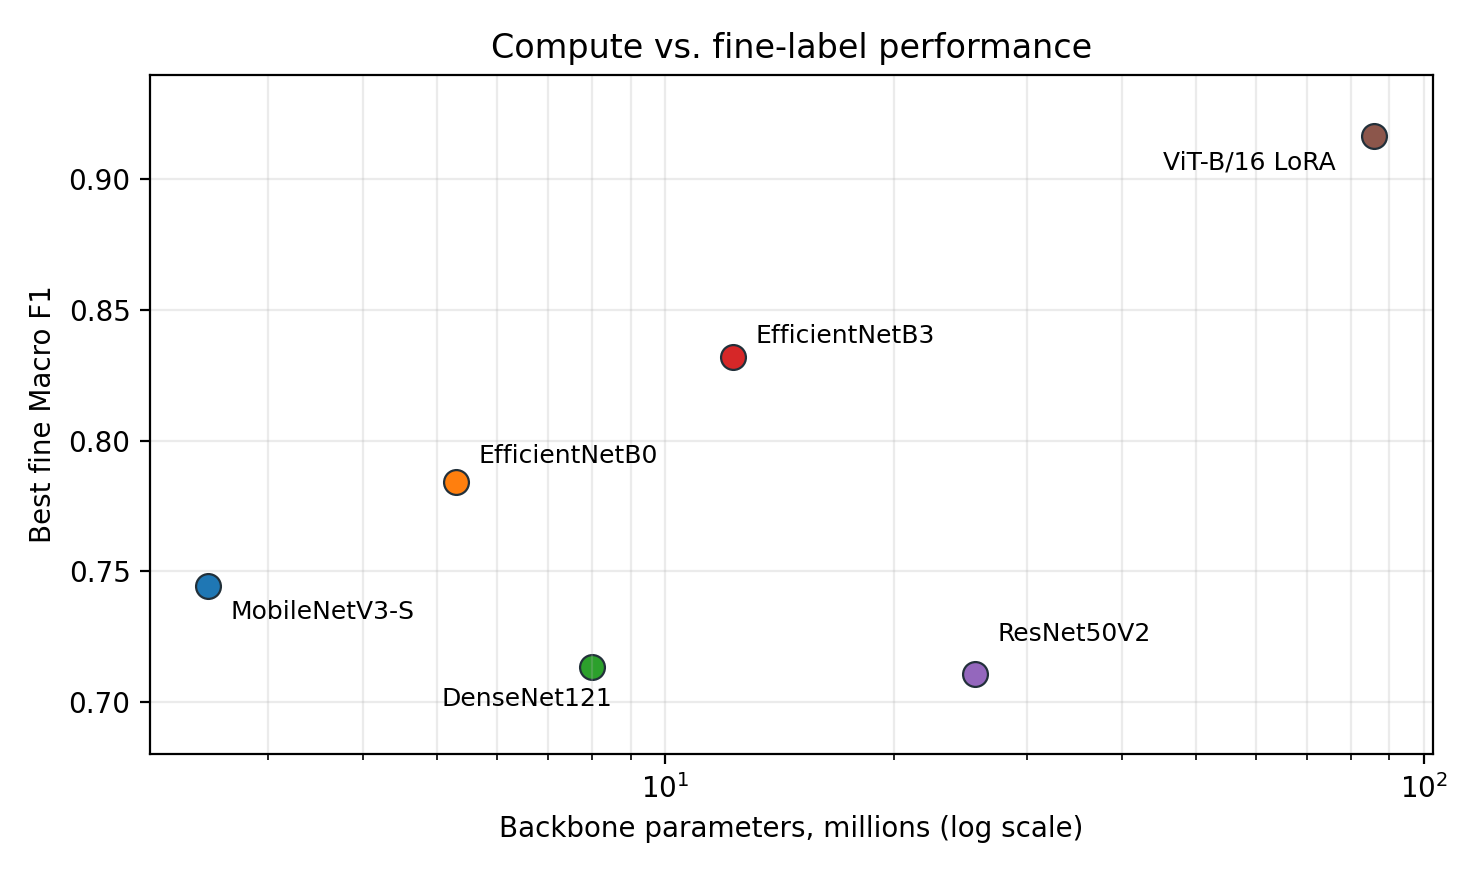
\includegraphics[width=\linewidth]{compute_vs_accuracy.png}
    \column{0.36\textwidth}
      \begin{itemize}
        \item Best fine Macro F1 against backbone size reveals a clear
              \textbf{Pareto frontier}.
        \item \textbf{MobileNetV3-S} is the value pick (2.5\,M, 0.74);
              \textbf{EfficientNetB3} the sweet spot (12.3\,M, 0.83).
        \item \textbf{ViT-B/16 LoRA} is the fine-task leader (Macro F1 0.917), but it
              also changes framework, input resolution, and pretraining scale.
      \end{itemize}
  \end{columns}
  \vfill
  \source{Parameters: standard published backbone sizes; F1 from local metrics and nb09.}
\end{frame}


% ----- 17 Conclusions: the whole comparison on one slide -----
\begin{frame}{Conclusions: one table, every architecture}
  \centering
  \footnotesize
  \renewcommand{\arraystretch}{0.9}
  \setlength{\tabcolsep}{4pt}
  \begin{tabular}{@{}lcccc@{}}
    \toprule
     & \textbf{Binary F1} & \textbf{Coarse F1} & \textbf{Fine F1} & \textbf{Family} \\
    \textbf{Architecture} & {\footnotesize(1-vs-rest)} & {\footnotesize(20 cls)} & {\footnotesize(100 cls)} & {} \\
    \midrule
    \arch{Baseline CNN}    & 0.60 & 0.26          & ---           & scratch  \\
    \arch{Strong CNN}      & ---  & 0.274         & ---           & scratch  \\
    \arch{Bi-LSTM}         & ---  & 0.345         & ---           & scratch  \\
    \arch{MobileNetV3-S}   & ---  & \best{0.841}  & 0.745         & transfer  \\
    \arch{EfficientNetB0}  & ---  & 0.739         & 0.784         & transfer  \\
    \arch{DenseNet121}     & 0.77 & 0.775         & 0.713         & transfer  \\
    \arch{EfficientNetB3}  & ---  & ---           & 0.832         & transfer \\
    \arch{ResNet50V2}      & 0.91 & 0.824         & 0.711         & transfer \\
    \arch{ViT-B/16 LoRA}   & ---  & ---           & \best{0.917}  & transformer \\
    \bottomrule
  \end{tabular}

  \vspace{0.15em}    % fmt: trimmed to clear vertical overflow
  \begin{columns}[T,onlytextwidth]
    \column{0.5\textwidth}
      \begin{itemize}
        \item \textbf{Coarse winner:} MobileNetV3-S (0.841) --- smallest \emph{pretrained} backbone wins coarse.
        \item \textbf{Fine winner:} ViT-B/16 LoRA (0.917); best ConvNet is EfficientNetB3 (0.832).
      \end{itemize}
    \column{0.5\textwidth}
      \begin{itemize}
        \item Fine-tuning usually improves the exported transfer runs; capacity matters most on fine labels.
        \item Bigger is not automatically better; ResNet50V2 is large yet mid-pack on fine.
      \end{itemize}
  \end{columns}
  \vspace{0.05em}    % fmt: trimmed to clear vertical overflow
  \source{Best Macro F1 per task from exported metrics; binary column = most separable 1-vs-rest class.}
\end{frame}


% ----- 18 Future work -----
\begin{frame}{Future work}
  \begin{columns}[T,onlytextwidth]
    \column{0.5\textwidth}
      \textbf{Modeling extensions}
      \begin{itemize}
        \item \textbf{Stronger sequence studies} --- tune row-wise LSTM/Bi-LSTM and compare
              against patch-sequence variants.
        \item \textbf{ViT from scratch} --- quantify exactly how much of the
              transformer's lead is ImageNet pretraining rather than architecture.
        \item \textbf{Parameter-efficient tuning} --- repeat the LoRA setting with
              multiple seeds and other transformer backbones.
      \end{itemize}
    \column{0.5\textwidth}
      \textbf{Sharper evaluation}
      \begin{itemize}
        \item \textbf{Augmentation study} --- a controlled grid (none $\to$ light $\to$
              strong) instead of a single fixed recipe.
        \item \textbf{Per-class thresholds} --- tune decision thresholds for the
              imbalanced 1-vs-rest tasks rather than a flat 0.5.
        \item \textbf{Multi-seed runs} --- error bars on the headline numbers and on any
              ViT and transfer-CNN deltas.
      \end{itemize}
  \end{columns}
  \vfill
  \begin{block}{One-line takeaway}
    Transfer learning makes CIFAR-100 tractable; the open questions are \emph{efficiency}
    and \emph{robustness}, not raw accuracy.
  \end{block}
\end{frame}


% ----- 19 Thank you / Q&A -----
\begin{frame}{Thank you}
  \vfill
  \centering
  {\Large\textbf{Questions \& Discussion}}\\[1.2em]

  \begin{columns}[c,onlytextwidth]
    \column{0.46\textwidth}
      \centering
      \textbf{Architectural Comparison\\on CIFAR-100}\\[0.4em]
      \source{Binary $\cdot$ Coarse (20) $\cdot$ Fine (100)\\CNN and Transformer families}
    \column{0.46\textwidth}
      \centering
      {\footnotesize Code \& full results:}\\[0.5em]
      \texttt{github.com/Fgram-devAI/}\\
      \texttt{deepl-cifar100-image-analysis}
  \end{columns}

  \vfill
  \source{MSc in Artificial Intelligence --- NCSR ``Demokritos'' \& University of Piraeus.}
\end{frame}


% ===== backup / appendix material =====
\appendix


% ----- backup: augmentation & evaluation notes -----
\begin{frame}{Backup: augmentation \& evaluation notes}
  \footnotesize    % fmt: match the other backup slides' size; clears overflow
  % fmt: itemize body template is globally \small; override locally so the dense
  % two-column notes fit. Scoped to this frame only.
  \setbeamertemplate{itemize/enumerate body begin}{\footnotesize}
  \begin{columns}[T,onlytextwidth]
    \column{0.5\textwidth}
      \textbf{Why light augmentation}
      \begin{itemize}
        \item CIFAR-100 images are only 32$\times$32 --- aggressive crops or large
              rotations destroy already-scarce detail.
        \item Flip + small shift/zoom/rotate gave a consistent small lift; heavier
              recipes hurt the baseline CNN.
        \item Augmentation was applied to \textbf{training only}; validation and test
              kept the clean upscaled image.
      \end{itemize}
      \vspace{0.4em}
      \textbf{Input-size handling}
      \begin{itemize}
        \item From-scratch controls use the native 32$\times$32 image or row-sequence view.
        \item EfficientNet runs resize to 96--160\,px; MobileNetV3, ResNet50V2,
              DenseNet121, and ViT use 224\,px.
        \item ViT uses its HF processor at 224\,px, so compare it as a standalone
              transformer result rather than a Keras-run clone.
      \end{itemize}
    \column{0.5\textwidth}
      \textbf{Evaluation choices}
      \begin{itemize}
        \item \textbf{Macro F1} as the headline metric: every class counts equally,
              unlike accuracy under 1-vs-rest imbalance.
        \item Binary tasks report F1 at a \textbf{validation-tuned threshold}, not a
              flat 0.5 --- the threshold metrics are stored per run.
        \item Top-5 accuracy reported alongside for the multiclass tasks.
      \end{itemize}
      \vspace{0.4em}
      \textbf{Honest caveats}
      \begin{itemize}
        \item Single seed (42) for the headline numbers --- no error bars yet.
        \item Parameter counts are standard published backbone sizes (Keras / HF).
      \end{itemize}
  \end{columns}
\end{frame}


% ----- backup: full binary (1-vs-rest) per-class results -----
\begin{frame}{Backup: binary 1-vs-rest, full per-class results}
  \footnotesize
  \begin{columns}[T,onlytextwidth]
    \column{0.5\textwidth}
      \centering
      \textbf{Baseline CNN --- best F1 per class}\\[0.3em]
      \renewcommand{\arraystretch}{1.15}
      \begin{tabular}{@{}lcc@{}}
        \toprule
        Target class & F1 & Acc \\
        \midrule
        \multicolumn{3}{@{}l}{\itshape coarse superclass (1-vs-rest)}\\
        flowers          & 0.574 & 0.953 \\
        food\_containers  & 0.487 & 0.934 \\
        people           & 0.491 & 0.950 \\
        fish             & 0.382 & 0.925 \\
        aquatic\_mammals  & 0.360 & 0.923 \\
        \midrule
        \multicolumn{3}{@{}l}{\itshape fine class (1-vs-rest)}\\
        skyscraper       & 0.600 & 0.992 \\
        orange           & 0.403 & 0.982 \\
        mushroom         & 0.268 & 0.989 \\
        cow              & 0.213 & 0.987 \\
        snake            & 0.149 & 0.964 \\
        \bottomrule
      \end{tabular}
    \column{0.5\textwidth}
      \centering
      \textbf{Transfer backbones --- same targets}\\[0.3em]
      \renewcommand{\arraystretch}{1.15}
      \begin{tabular}{@{}lcc@{}}
        \toprule
        Run & F1 & Acc \\
        \midrule
        ResNet50V2 skyscraper, ft   & \best{0.910} & 0.998 \\
        ResNet50V2 skyscraper, fr   & 0.809 & 0.996 \\
        DenseNet121 skyscraper, fr  & 0.773 & 0.996 \\
        ResNet50V2 food\_cont., fr   & 0.843 & 0.984 \\
        ResNet50V2 orange, fr       & 0.833 & 0.997 \\
        \bottomrule
      \end{tabular}\\[1.0em]
      \raggedright
      \textbf{The imbalance illusion.} Every baseline row clears
      $\sim$92--99\% \emph{accuracy} while F1 stays low: the model mostly
      predicts ``not target''. Transfer learning lifts the \emph{same}
      skyscraper target from F1 0.60 to \best{0.91}.\\[0.4em]
      \source{fr = frozen head, ft = fine-tuned; best run per class shown.}
  \end{columns}
\end{frame}


% ----- backup: fine confusion detail + ViT provenance -----
\begin{frame}{Backup: fine confusion structure (EfficientNetB3)}
  \begin{columns}[T,onlytextwidth]
    \column{0.50\textwidth}
      % fmt: height cap leaves room for the source line below the square matrix
      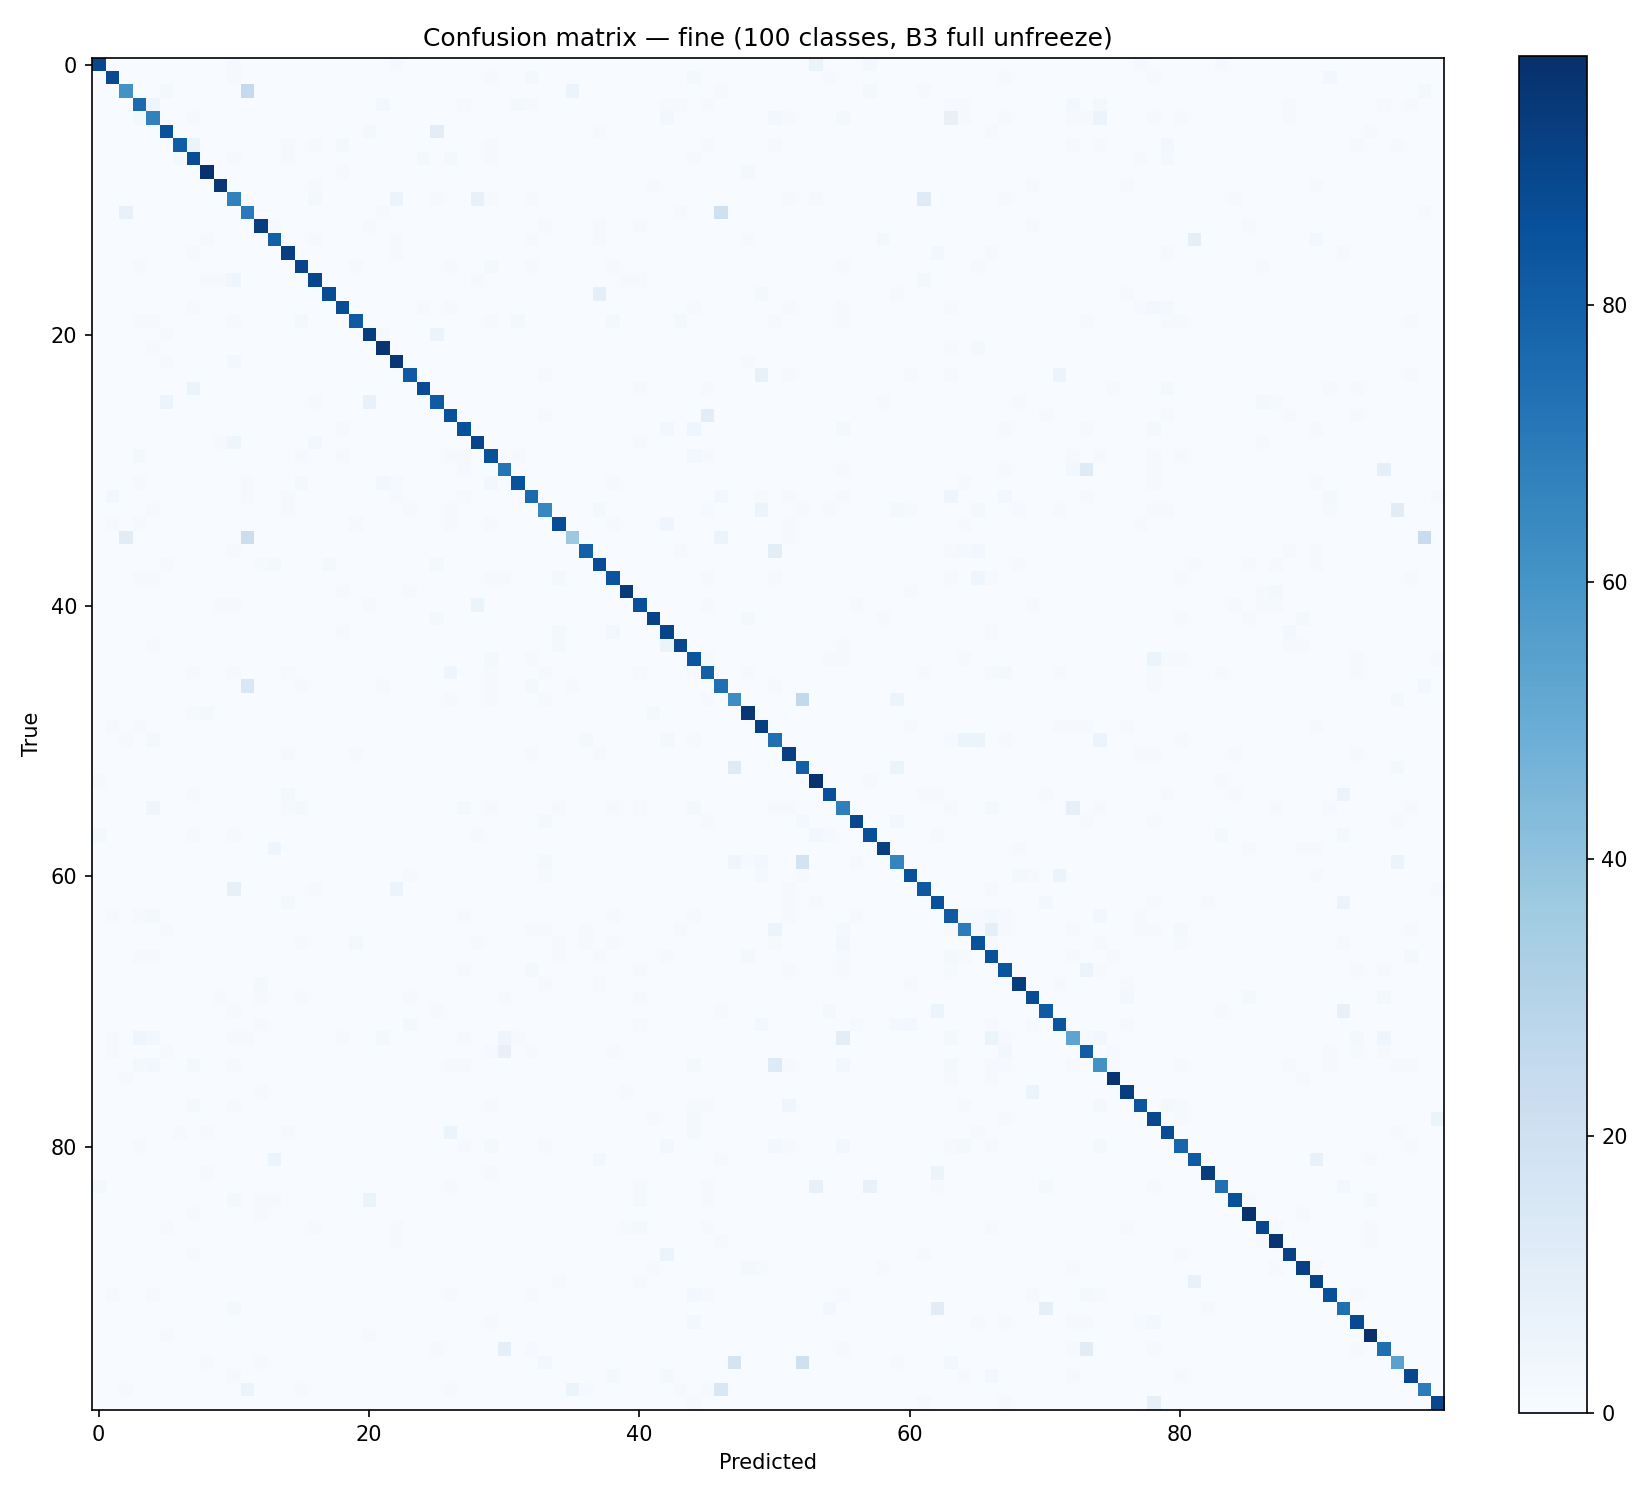
\includegraphics[width=0.96\linewidth,height=0.68\textheight,keepaspectratio]{efficientnetb3_fine_confusion.png}\\
      \source{nb08 EfficientNetB3 fine, full fine-tune (best ConvNet).}
    \column{0.46\textwidth}
      \footnotesize
      \begin{itemize}
        \item The 100$\times$100 matrix is \textbf{strongly diagonal}; off-diagonal
              mass sits \emph{within} superclasses.
        \item Residual errors are semantic neighbours --- maple\,$\leftrightarrow$\,oak,
              boy\,$\leftrightarrow$\,man.
        \item This is why \textbf{coarse} accuracy outruns \textbf{fine}: the hard
              confusions live inside the superclass.
      \end{itemize}
      \vspace{0.4em}
      \begin{block}{Provenance --- ViT (nb09)}
        {\scriptsize nb09 is a standalone Hugging Face ViT workflow. The reported
        LoRA result reaches Macro F1 0.9165 and Top-5 0.9919 on the fine test
        split, using a different framework stack, resize policy, and training loop
        from the TensorFlow/Keras transfer runs.}
      \end{block}
  \end{columns}
\end{frame}


% ----- backup: ViT run summary -----
\begin{frame}{Backup: ViT run summary}
  \footnotesize
  \begin{tabular}{@{}lrrrr@{}}
    \toprule
    \textbf{Run} & \textbf{Accuracy} & \textbf{Macro F1} & \textbf{Top-3} & \textbf{Top-5} \\
    \midrule
    Frozen head      & 0.8628 & 0.8629 & 0.9538 & 0.9719 \\
    Partial fine-tune& 0.8874 & 0.8873 & 0.9690 & 0.9812 \\
    LoRA             & 0.9165 & 0.9165 & 0.9831 & 0.9919 \\
    \bottomrule
  \end{tabular}
  \vspace{0.8em}
  \begin{itemize}
    \item The LoRA run loads from the Run A trained checkpoint and trains attention
          projection adapters (`q\_proj`, `k\_proj`, `v\_proj`).
    \item The result should be described as a Hugging Face/PyTorch transformer
          result, not as part of the TensorFlow/Keras transfer pipeline.
  \end{itemize}
  \vfill
  \source{nb09 final summary table and printed trainable-parameter report.}
\end{frame}


% ----- backup: hyperparameters of the headline runs -----
\begin{frame}{Backup: hyperparameters of the headline runs}
  \centering
  \footnotesize
  % fmt: itemize body template is globally \small; override locally so the dense
  % two-column notes fit and the source line clears the footer. Scoped to this frame.
  \setbeamertemplate{itemize/enumerate body begin}{\footnotesize}
  \renewcommand{\arraystretch}{1.08}    % fmt: trimmed from 1.2 to clear overflow
  \setlength{\tabcolsep}{5pt}
  \begin{tabular}{@{}lccccc@{}}
    \toprule
    \textbf{Run} & \textbf{Input} & \textbf{Epochs} & \textbf{LR} & \textbf{Batch} & \textbf{Regime} \\
    \midrule
    Baseline CNN (coarse)      & 32  & 50 & 3e-5 & 64 & from scratch \\
    Bi-LSTM (coarse)           & 32 rows & 20 & 1e-3 & 128 & from scratch \\
    Strong CNN (coarse)        & 32  & 45 & 3e-5 & 128 & aug. + regularized \\
    MobileNetV3-S (coarse)     & 224 & 30 + 20 & 1e-3 / 1e-5 & 32 & frozen $\to$ unfreeze \\
    EfficientNetB0 (fine)      & 128 & 30 / 30 / 40 & 1e-3 / 1e-4 / 1e-5 & 64 & frozen $\to$ block6 $\to$ full \\
    EfficientNetB3 (fine)      & 160 & 40 & 1e-5 & 16 & full fine-tune \\
    ResNet50V2 (coarse/fine)   & 224 & 20 + 5 & 1e-4 / 2e-6 & 32 & frozen $\to$ fine-tune \\
    DenseNet121 (coarse/fine)  & 224 & 20 + 5 & 1e-4 / 2e-6 & 32 & frozen $\to$ fine-tune \\
    ViT-B/16 (fine)            & 224 & 5 each & 3e-4 / 3e-5 / 1e-4 & 16--32 & HF notebook \\
    \bottomrule
  \end{tabular}

  \vfill
  \begin{columns}[T,onlytextwidth]
    \column{0.5\textwidth}
      \textbf{Shared recipe}
      \begin{itemize}
        \item Optimiser \textbf{Adam}; loss categorical cross-entropy (BCE for binary).
        \item Dropout and augmentation are configured per run.
        \item Early stopping monitor varies by experiment; fixed \textbf{seed 42} where configured.
      \end{itemize}
    \column{0.5\textwidth}
      \textbf{Light augmentation (when enabled)}
      \begin{itemize}
        \item Horizontal flip plus small translation, zoom, rotation, and contrast.
        \item Strong CNN used a light regularized augmentation recipe.
        \item 10\% validation split held out of the 50k training set.
      \end{itemize}
  \end{columns}
  \vfill
  \source{Representative values from exported config snapshots and local YAML files.}
\end{frame}


\end{document}
